\documentclass[12pt]{article}
\usepackage{amsmath,amsthm}
\usepackage[utf8]{inputenc}
%\usepackage[T1]{fontenc}
%\usepackage{minionpro}
\usepackage{array,graphicx}
\usepackage{chicago}        %bibliography style
\usepackage{booktabs}       %to make table lines thicker
\usepackage{dcolumn}

\setlength{\topmargin}{-0.3in} \setlength{\textheight}{8.75in}
\setlength{\oddsidemargin}{0.25in} \setlength{\evensidemargin}{0.25in}
\setlength{\textwidth}{6in}
\def\labelenumi{\arabic{enumi}.}
\def\theenumi{\arabic{enumi}}
\def\labelenumii{(\alph{enumii})}
\def\theenumii{\alph{enumii}}
\def\p@enumii{\theenumi.}
\def\labelenumiii{\arabic{enumiii}.}
\def\theenumiii{\arabic{enumiii}}
\def\p@enumiii{(\theenumi)(\theenumii)}
\def\labelenumiv{\arabic{enumiv}.}
\def\theenumiv{\arabic{enumiv}}
\def\p@enumiv{\p@enumiii.\theenumiii}
\pagestyle{plain}
\pagestyle{plain} \setcounter{secnumdepth}{3}
\newcommand{\D}{\mathop{\mathrm{d\mathstrut}}\nolimits\!}
\newcommand{\dt}{\D t}
\newcommand{\dz}{\D z}
\newcommand{\E}{\mathop{\mathrm{E\mathstrut}}\nolimits}
\newcommand{\Var}{\mathop{\mathrm{Var\mathstrut}}\nolimits}
\newcommand{\sd}{\mathop{\mathrm{sd\mathstrut}}\nolimits}
\newcommand{\diag}{\mathop{\mathrm{diag\mathstrut}}\nolimits}
\newcommand{\Cov}{\mathop{\mathrm{Cov\mathstrut}}\nolimits}
\newcommand{\Corr}{\mathop{\mathrm{Corr\mathstrut}}\nolimits}
\newtheorem{definition}{Definition}
\newtheorem{proposition}{Proposition}
\newtheorem{conjecture}{Conjecture}
\newtheorem{moment}{Empirical regularity}
\newtheorem{insight}{Qualitative prediction}

\renewcommand{\baselinestretch}{1.17}

\newcommand{\dofigure}[3]{\begin{figure}
\begin{centering}
\includegraphics[width=0.75\linewidth]{figures/#1}
  \caption{#2\label{fig:#1}}
\end{centering}

\noindent \footnotesize{#3}
\end{figure}}

\newcommand{\dotable}[2]{\begin{table}[h!]
\begin{centering}
\caption{#2\label{tab:#1}}
\includegraphics[width=0.75\linewidth]{figures/#1}
\end{centering}
\end{table}}

\begin{document}

\title{Cattle, Steaks and Restaurants:\\ Development Accounting when Space Matters\thanks{For useful comments, we thank Thomas Holmes, Esteban Rossi-Hansberg, Albert Saiz, Adam Szeidl, Jonathan Vogel, Kei-Mu Yi and seminar audiences. The views expressed here are our own and do not reflect those of the ECB and the Eurosystem.}}
\author{Péter Karádi\thanks{European Central Bank. E-mail: peter.karadi@ecb.int} and Miklós Koren\thanks{Central European University, MTA KRTK and CEPR. E-mail: korenm@ceu.edu.}}
\maketitle

\begin{abstract}
We introduce location choice in a multi-sector general equilibrium model to study how it affects development accounting. Producers in agriculture, manufacturing and services choose their location to trade off land rents with transport costs to the city center. We show how space affects the aggregate production function and decompose output per worker into productivity, land per worker, and a term adjusting for sector location. In our model, services are luxury goods. As a result, richer cities have larger service cores, higher service prices, and relatively less output per worker in services. These predictions are broadly consistent with the data. We calibrate our model to data on cities in OECD countries and show that land and location explain 10--30 percentage points of the variation in output per worker.
\end{abstract}

Output per worker is much lower in poor countries than in rich ones \cite{Klenow97,Hall99,Caselli05}. To understand the fundamental causes of productivity differences, it is important to identify the sectors in which these differences are the greatest. Several recent papers have studied the sectoral composition of productivity differences by using data on sector-level inputs, outputs and prices \cite{Bailey01,Caselli05,Restuccia08,Duarte10,Duarte2015-gl}. Their main result is that productivity differences are sizeable and they are larger in agriculture than in manufacturing and services.\footnote{These results are in line with the classic Balassa-Samuelson literature \cite{Balassa64,Samuelson64,Baumol65,Baumol67}, which explains sectoral price-level differences by productivity advantage of manufacturing over services.}

Labor productivity depends on the quantity or quality of inputs used in the production process. Here we argue that land input has been conspicuously missing from development accounting exercises to date. Controlling for land when estimating macro productivity is important for two reasons. First, countries with high population density are relatively scarce in land and, to the extent that land matters in production, these countries will have low labor productivity. Second, land varies in a crucial quality component: its proximity to consumers. Urban land is more valuable because it is more productive in producing goods and services with high transport costs. Again, countries may differ in the availability of urban land. Accounting for land and location is especially important for sector-level development accounting. Agriculture uses land intensively and will be especially sensitive to controlling for the quantity of land. Services, in turn, locate in urban areas and will be especially sensitive to controlling for location.

To understand how land and location affect development accounting, we build a simple multi-sector general equilibrium model. Each sector uses labor (or a composite of other spatially mobile inputs) and land. The location of sectors is determined as in the canonical von Thünen city model. In the model, all trade happens in the city center, the central business district (CBD). Producers choose their location freely on a plane, and have to pay a shipping cost to transport their goods to the CBD. This spatial structure introduces variable land-quality to the model, as land closer to the CBD saves on transport cost. Equilibrium rents decrease with distance from the CBD, and the producers optimally choose locations to balance savings on transport costs with higher rents. Our model yields a simple spatial equilibrium in which agriculture (``cattle'') locates farthest away from the center, manufacturing (``steaks'') occupies a ring outside the center, and services (``restaurants'') are in a central circle.

We can decompose output per worker into three components: (i) Hicks neutral productivity (which will also capture the presence of spatially mobile factors such as capital), (ii) land per worker, and (iii) a term reflecting distance to consumers. Components (ii) and (iii) are novel to our model. First, as some sectors are more land intensive, their labor productivity will be more sensitive to the scarcity or abundance of land. Conditional on other productivity factors, agricultural output per worker will be higher in countries with an abundant supply of land. Second, urban sectors (such as services) will be relatively more productive in smaller cities where transport costs are lower.

To quantify the importance of these two mechanisms, we calibrate our model to city-level data on employment density, city size, and GDP per capita (from the OECD Metropolitan Areas Database) and country-level prices and expenditure shares (from the International Comparison Program). We set common technology parameters to match the sectoral land-shares and spatial distribution of economic activities in the U.S. We then use the calibrated model to decompose output per worker into the three components for each city.

Perhaps unsurprisingly, the largest variation across cities in output per worker is due to variation in Hicks neutral productivity. We estimate this productivity variation to be essentially the same in the three broad sectors. This is in contrast with the existing literature, which finds more variation agricultural productivity \cite{Caselli05,Restuccia08},\footnote{Admittedly, data on metropolitan areas is less informative about productivity in agriculture than in the two other sectors.} and less variation in services productivity \cite{Balassa64,Samuelson64,Herrendorf2012-yg}.\footnote{\citeN{Duarte2015-gl} find that productivity in tradable business services varies more than in manufacturing.}

Variation in land per worker explains up to 30 percentage points of productivity differences across the cities in our sample. This variation is biggest in agriculture, which uses land intensively. In our sample, land per worker does not vary systematically with development.

Sector location explains up to 10 percentage points of productivity differences. This varies systematically with development as poorer cities spend less on services and have smaller service cores. Transportation costs in these cities is lower and output per worker is higher.

More broadly, our model illustrates how to incorporate space in a simple development accounting model and that transport costs can have macro relevance. In related work, \citeN{Ramondo2016-qy} incorporate space in a macro model with transport costs, arguing that large countries have larger transport costs and hence not as high GDP per capita. The main difference is that while \citeN{Ramondo2016-qy} capture average trade costs across cities within a country, our main focus is the within-city trade cost and spatial structure. Also related are \citeN{Desmet2013}, who study an endogenous system of cities (in our work, cities are exogenous in size) and \citeN{Desmet2014-nh}, who study cities and growth (our model is static). Neither of these papers focus on the spatial allocation of sectors as we do. \citeN{Adamopoulos11} analyzes the impact of lower transport costs in rich countries on their productivity advantage. He finds that lower transport costs can reduce missallocation, improve agriculture productivity and lead to the reallocation of labor away from agriculture.\footnote{See also \citeN{Gollin14,Adamopoulos14}.} Differently from him, our focus is on the heterogeneity in transport cost across sectors and its impact on structural transformation and urbanization.

\citeN{Lagakos2013-da} study a model of structural change where workers vary in agricultural productivity. In poor countries, more people will work in agriculture, and their average productivity will be low. Our model features a similar mechanism, but in our setting, it is the productivity of land that is heterogeneous, as it depends on distance to the center. In rich countries, more land will be devoted to services, resulting in relatively lower output per worker.

Heterogeneous land quality contributes also to the reallocation of labor towards urban sectors, usually referred to as structural transformation (for a recent review, see \citeN{Herrendorf14}). Development increases the relative demand for the more luxury urban goods \cite{Echevarria97,Kongsamut01,Gollin02}. This increases the scarcity of urban land, and forces urban sectors to substitute towards labor. Furthermore, the increasing price of urban land raises the relative price of urban sectors, and modifies the measurement of relative technological growth. Our estimation suggests that technology grows relatively faster in rural sectors \cite{Ngai07,Restuccia08}, and this exerts an additional force towards structural transformation [FIXIT: does it?].

Our model is motivated by four robust empirical facts. First, urban land becomes more important with development relative to rural land \cite[Figure 10.3]{Clark}. Second, the relative price of services increase with development. This is known as Baumol's cost disease \cite{Baumol65} or the Balassa-Samuelson effect \cite{Balassa64,Samuelson64}. Third, rich countries are more urbanized \cite{United_Nations2014-zm}. Fourth, rich countries produce less agriculture and more services \cite{Kuznets1973,Ngai2007,Kongsamut01}. As we show below, our model is capable of explaining these facts in a simple framework.


\section{A model of industry location}
We introduce location choice in a multi-sector general equilibrium model. We have two sectors: urban and rural, each using land and labor for production. Our spatial structure follows the von Thünen monocentric city model: producers choose a location on the plane and need to transport their goods to the central business district.

A city is a point on a bounded but otherwise featureless two-dimensional plane. A country is a collection multiple cities, with goods and people moving freely across these cities. We assume that countries are large enough such that city boundaries never overlap with each other or with country boundaries.

We first characterize the distribution of economic activities within a city, then discuss equilibrium allocation across cities within a country.

\subsection{Consumers}
To be consistent with Fact 4, we assume non-homothetic consumer preferences. We follow \citeN{Fieler11} in assuming an isoelastic utility function with different elasticities for the three sectors.\footnote{We have estimated the preferences proposed by \citeN{Kongsamut01}, \citeN{Ngai2007} and \citeN{Herrendorf2013} on cross-country data, but this provided a poor fit for rich countries, where the role of necessity spending is vanishingly small.}

A consumer living in city $c$ enjoys utility
\begin{equation}
\label{eq:Utility}
u_c = 
\alpha_u^{1/\sigma_u}
	\frac {\sigma_u}
			{\sigma_u-1}
	C_{cu}^{1-1/\sigma_u}
	+
	\frac {\sigma_r}
			{\sigma_r-1}
	C_{cr}^{1-1/\sigma_r},
\end{equation}
where $\alpha_u>0$ is the weight of the urban sector (we have normalized $\alpha_r=1$) and $\sigma_i>1$ governs the sector's price and income elasticity. Sector $u$ refers to ``urban goods,'' $r$ refers to ``rural goods.'' 

There is a mass $N$ of consumers who supply one unit of labor inelastically, and rent land to producers in a competitive market. They are \emph{absentee landlords}: the rents they collect are independent of the place of employment.

The budget constraint of a city-$c$ consumer is
\begin{equation}
\label{eq:BudCons}
P_u C_u + P_r C_r
	= W_c + R/N,
\end{equation}
where $W_c$ is the wage level in city $c$ and $R$ is the total rent in the economy.

The sectoral consumption expenditures satisfy
\begin{equation}\label{eq:ConsShares}
{P_i c_i}
=
\alpha_i
\lambda^{ - \sigma_i}
{ P_i^{1-\sigma_i}},
\end{equation}
where $\lambda$ is the Lagrange multiplier of the budget constraint, which is decreasing in income. For a given set of prices, the expenditure of good $u$ relative to good $r$ is increasing in income if $\sigma_u>\sigma_r$.
The income elasticity of good $i$ is
\begin{equation}\label{eq:income_elasticity}
\frac 	{\partial \ln c_i}
		{\partial \ln y}
=
\frac 	{\sigma_i}
		{\sum_j x_j\sigma_j},
\end{equation}
where $x_j=P_jc_j/\sum_k P_kc_k$ is the expenditure share of good $j$.


\subsection{Producers}
Output in sector $i$ at location $z$ depends on labor $N$ and land $L$ used at that location,
\[
Q_i(z) =\beta^{-\beta}(1-\beta)^{-(1-\beta)} A_i L_i(z)^{\beta}N_i(z)^{1-\beta}.
\]
We take labor to be freely mobile within the city, land is in fixed $\Bar{L}(z)$ supply in each location. The names ``land'' and ``labor'' are for the sake of convenience, these two factors correspond to spatially fixed and mobile factors, respectively, and we will calibrate them accordingly.\footnote{For analytical convenience, we assume that both sectors have the same land intensity $\beta$. This will ensure that the overall national wage level does not affect city size. In practice, rural sector have a somewhat higher land intensity. The qualitative conclusions of our model are the same in this case.}

Products are sold at a single marketplace in each city, the central business district. This is location $z=0$, so that $z$ indexes distance to the center. We will first characterize the spatial equilibrium in one city, then discuss the equilibrium across multiple cities within a country.

There are two sectors, urban and rural. The urban sector has a shipping cost, rural sector has not.
To ship an urban product to the center, one has to incur shipping costs. If a unit of product leaves location $z$, only
\[
e^{-\tau z}
\]
units arrive at the center. We assume that once a good arrives at the center, it can be freely traded across cities. This ensures that the law of one price holds across cities, and is a convenient simplification driven by the fact that we have no data on city-level prices.\footnote{An alternative interpretation of transport costs within the city is that production takes place at the CBD, while workers have to commute from farther away. In this case, $\tau$ captures commuting costs.}

In the rural sector, goods can be shipped freely. This will ensure that in equilibrium agricultural goods are produced outside cities in rural areas.

Profits from production at $z$ are
\begin{equation}
\label{eq:profit}
\Pi_u(z)=P_ue^{-\tau z}Q_u(z)-W_uN_u(z)-R_u(z)L_u(z)
\end{equation}
for the urban sector and
\begin{equation}
\label{eq:profit:rural}
\Pi_r(z)=P_r Q_r(z)-W_rN_r(z)-R_rL_r(z)
\end{equation}
for the rural sector. A sector being active at location $z$ requires that their maximized profit $\max\Pi(z)\geq0$.

\subsection{Spatial Sorting}
Because space if featureless, the available land at each distance $z$ from the CBD is $\Bar L(z) \equiv 2z\pi$. We study symmetric equilibria where the distance to the CBD completely characterizes a location.

\begin{definition}
Given a level of prices $P_u$, $P_r$ and wages $W$, define the \emph{spatial sorting} in a circular city as a set of quantities $Q_i(z), L_i(z), N_i(z)$ such that
\begin{enumerate}
    \item The producers choose location $z$, and nonnegative quantities $Q_i(z), L_i(z), N_i(z)$ to maximize their profits (\ref{eq:profit}), taking prices as given.
    \item Land markets clear at every location: $L_u(z)+L_r(z)=\Bar L(z)$ for all $z\in Z$.
\end{enumerate}
\end{definition}
The spatial sorting, as we show below, has a simple and intuitive structure. The urban sector with a positive transport cost intensity $\tau$ locates closer to the center. The rural sector is produced outside cities.

To see why this is the case, construct the sectoral bid rent curve $R_i(z)$. This is the maximum rent an active producer in the urban sector would be willing to pay at location $z$. %In a competitive market, the sector with the highest bid rent curve is active at a location ($R(z)=\max_iR_i(z)$ for all $z$).
A profit maximizing producer is choosing its land $L_i(z)$ and labor demand $N_i(z)$ to equalize the value marginal product of land and labor to rents and wages, respectively. It is true for any rent function or wages it might face, so it is true for rents given by its own bid-rent curve $R_i(z)$, in particular.
\begin{align}
R_i(z) &=\beta^{1-\beta}(1-\beta)^{-(1-\beta)} P_ie^{-\tau_i z}A_i \left(\frac{N_i(z)}{L_i(z)}\right)^{1-\beta}\\
W &=\beta^{-\beta}(1-\beta)^{\beta)} P_ie^{-\tau_i z}A_i \left(\frac{N_i(z)}{L_i(z)}\right)^{-\beta}
\end{align}
The sectoral labor-land ratio (employment density) can be expressed as
\begin{equation}
\label{eq:EmpDens}
\frac{N_i(z)}{L_i(z)} = \frac{1-\beta}{\beta}\frac{R_i(z)}{W}.
\end{equation}
Substituting this into the first-order condition for land use and rearranging, we get the bid rent curve:
\begin{equation}
\label{eq:BidRent}
R_i(z) =(P_iA_i)^{1/\beta} W^{1-1/\beta} e^{-\frac{\tau_i}{\beta} z}
\end{equation}
with $\tau_u=\tau$ for the urban sector and $\tau_r=0$ for the rural sector. Equation (\ref{eq:BidRent}) pins down the gradient of the sectoral rent curve, which determines how fast the bid-rents decrease with the distance from the CBD. The gradient is an increasing function of the transport cost and a decreasing function of land share $|\partial\log R(z)/\partial \log z|=\tau/\beta$. Intuitively, transport costs ($\tau z$) increase with distance, so producers offer lower rents for farther locations. If land were the only factor of production ($\beta=1$), only this direct effect would be present and the gradient would only depend on the transport cost intensity. With labor present, however, the producers can substitute labor for land, introducing an indirect effect on the gradient. As the equilibrium land-labor ratio shows (see equation \ref{eq:EmpDens}), the land share $\beta$ determines the strength of this substitutability: higher land share implies bid-rent curves decreasing with a slower rate.

Wherever the rural sector is active, it pays a fixed rent of
\[
R_r = (P_rA_r)^{1/\beta} W^{1-1/\beta}
\]
Because agricultural goods are freely tradable, their bid-rent does not depend on location.

We can also get the urban employment gradient by substituting the bid rent curve into the labor-land ratio,
\begin{equation}
\label{eq:EmpGrad}
\frac{N_u(z)}{L_u(z)} = \frac{1-\beta}{\beta} \left(\frac{P_uA_u}{W}\right)^{1/\beta} e^{-\frac{\tau}{\beta} z}.
\end{equation}
This is the relationship we use to calibrate the sectoral transport cost intensities.

\begin{proposition}\label{prop:existence}
There exists a competitive spatial equilibrium, characterized by location $0<z_u$ such that the urban sector produces at $\left[0,z_u\right]$, and agriculture locates in $(z_u,\infty)$.
\end{proposition}
The different exponential slope of the bid-rent curves ensures that they cross exactly once. This results in a strict partitioning across sectors, as shown in Figure \ref{fig:BidRent}.

\begin{figure}[h!]
\caption{Spatial equilibrium\label{fig:BidRent}}
\begin{center}
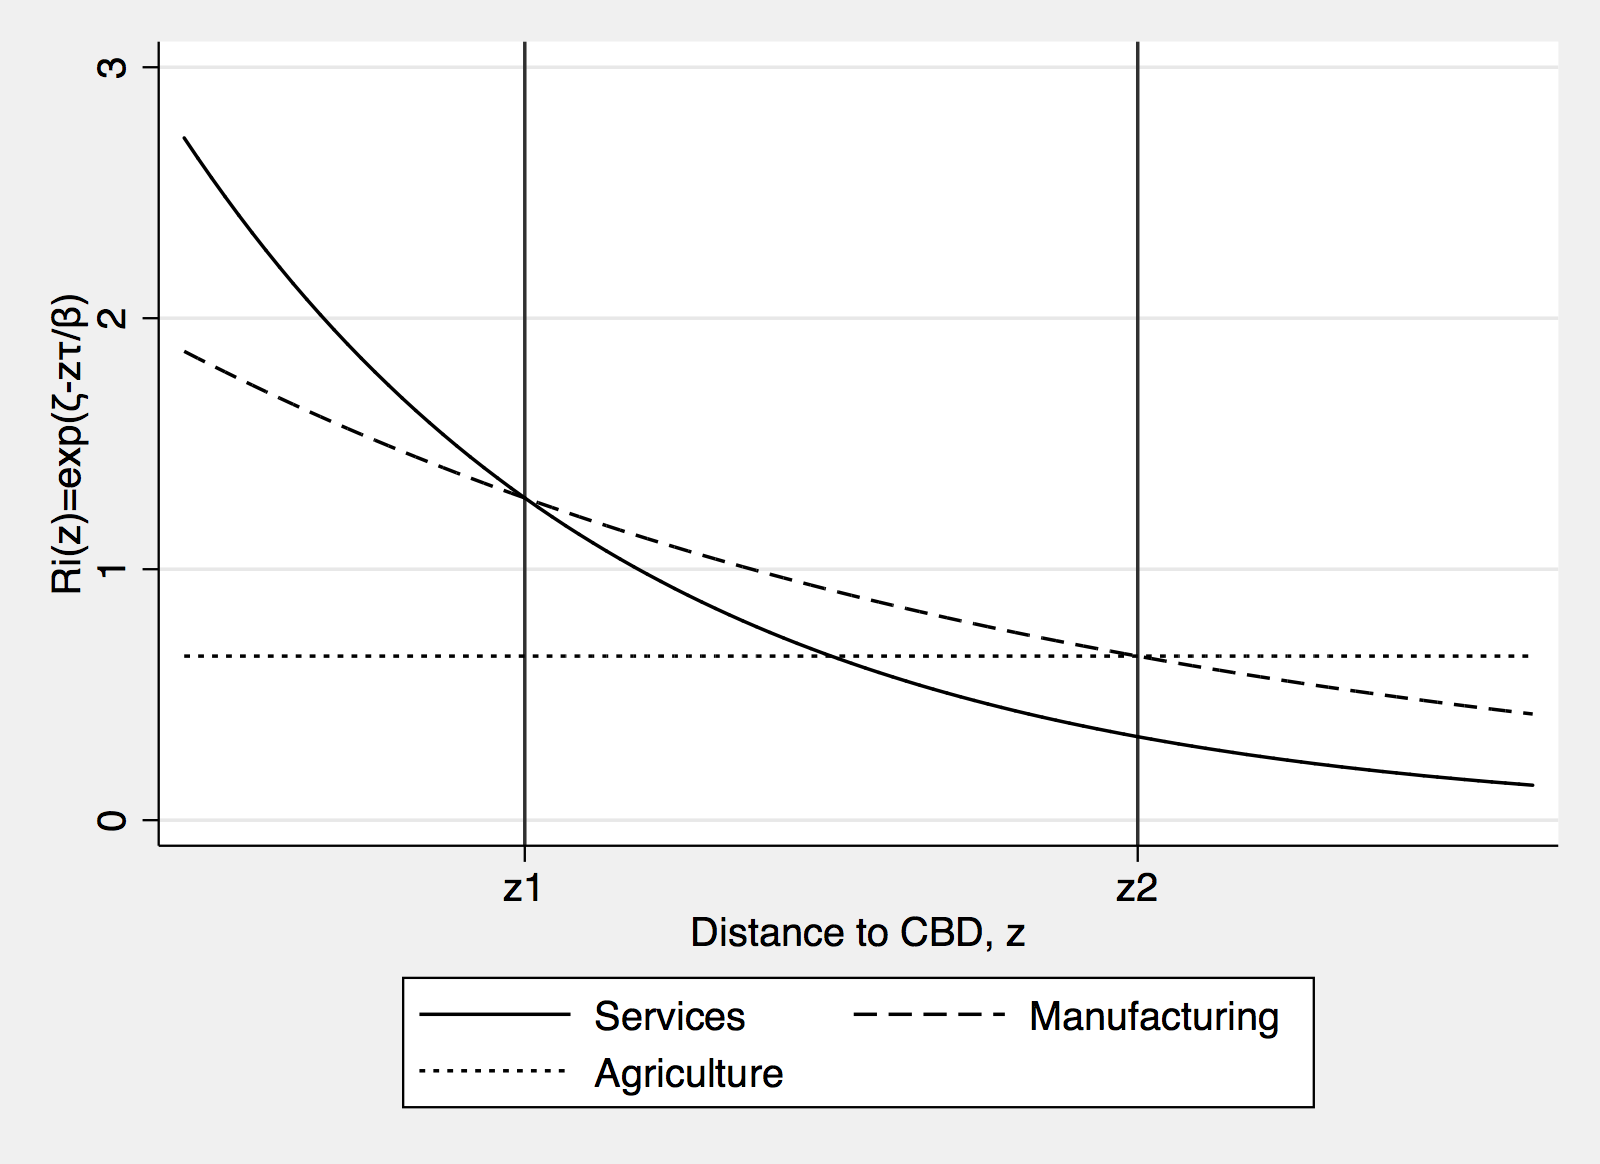
\includegraphics[scale=0.4]{figures/bid_rent_curves}
\end{center}

\noindent \footnotesize{The figure plots the structure of a competitive spatial equilibrium. It shows equilibrium sectoral bid rent curves as a function of distance from the city center. A sector is active over an area where it is willing to overbid the sector. Crossings of the bid-rent curves determine the borders of the sectors. The urban sector is active in $[0,z_u]$, agriculture in $(z_u,\infty)$.}
\end{figure}

Each city is characterized by a distance cutoff $z_u$. Locations $z>z_u$ cannot be associated with any particular city and we will call them agricultural or rural land. This implies that $z_u$ will be the functional city boundary and we will calibrate the model accordingly.

\subsection{Aggregation across space}
For the urban sector, production is a function of a suitably chosen representative location. Sectoral output measured at the center is
\begin{equation*}
\tilde{Q}_u=B\int_{z=0}^{z_u}e^{-\tau z}A_uL(z)^\beta N_u(z)^{1-\beta}dz,
\end{equation*}
with $B=\beta^{-\beta}(1-\beta)^{-(1-\beta)}$.

Let the representative location
\begin{equation}
\label{eq:ReprLoc}
\tilde z = -
\frac{\beta}{\tau}
\ln\int_{z=0}^{z_u} \frac{L(z)}{L_u}e^{-\frac{\tau}{\beta} z}dz
\end{equation}
denote the average distance of the urban sector to the center, where $L_u=\int_{z=0}^{z_u} L(z)dz$ is the total amount of land devoted within the city fringe. This definition ensures that the trade cost going to location $\tilde z$ equals the land-weighted average trade cost across all sectoral locations,
\[
e^{-\frac{\tau}{\beta} \tilde z} = \int_{z=0}^{z_u} \frac{L(z)}{L_u}e^{-\frac{\tau}{\beta} z}dz.
\]
As we will see below, $\tilde z$ is a sufficient statistic about sector location for aggregation purposes.

\begin{proposition}\label{prop:aggregation}
City-level production function is of the form:
\begin{equation}
\tilde Q_u =
BA_uL_u^{\beta}N_u^{1-\beta}
 e^{-\tau\tilde z}.
\end{equation}
It depends on trade costs from the representative location ($\tilde{z}$) defined by equation \eqref{eq:ReprLoc} and is a Cobb-Douglas aggregate of sectoral land ($L_u=\int_{z=0}^{z_u}L(z)dz$) and labor ($N_u=\int_{z=0}^{z_u}N(z)dz$) use.
\end{proposition}

Rent arbitrage between manufacturing and agriculture, $R_u(z_{u}) = R_{r}$, pins down the city boundary:
\begin{equation}\label{eq:city_boundary}
e^{z_{u} \tau} =
\frac {P_uA_u} {R_r^{\beta} W^{1-\beta}}
 =
\frac {P_uA_u}{P_rA_r}
\end{equation}
The size of the city increases in the relative price and relative productivity of urban goods. Intuitively, when cities are productive (either in price or quantity), they can outbid the rural sector for land. These cities will be larger. 

City employment density is
\begin{equation}\label{eq:city_employment}
\frac{N_u}{L_u} = \frac{1-\beta}{\beta} \left(\frac{P_uA_u}{W}\right)^{1/\beta} e^{-\tilde z\tau/\beta}
=\frac{1-\beta}{\beta}
	 \left(\frac{P_uA_u}{P_rA_r}\right)^{1/\beta}
	 \left(\frac{W}{P_rA_r}\right)^{-1/\beta}
	 e^{-\tilde z{\tau/\beta}}.
\end{equation}
For a given city area, employment is increasing in the relative price and relative productivity of the city and decreases in the wage rate. It also decreases in city size. More productive cities will pay higher average rent, so producers will substitue land for labor. The opposite will hold when wages are high. And city size decreases employment density because of a selection effect: the the typical plot of land in large cities will be cheaper land, far away from the center. These plots will make more intense use of land.

Equations \eqref{eq:city_boundary} and \eqref{eq:city_employment} completely characterize the spatial sorting within a city. City features depend on relative urban to rural productivity and a relative wage rate.

The primary object of interest is the rent curve plotted in Figure \ref{fig:BidRent}. Urban rents will always be higher than rural rents, because urban plots have a productivity advantage: they are closer to the center. Even though city boundaries are determined in frictionless equilibrium, rents are only equalized \emph{at the margin}. Rents at inframarginal urban locations command a premium. More specifically,
the ratio of urban to rural rent
\[
\frac{R_u}{R_r} = \frac{R(0)e^{-\tilde z \tau /\beta}} {R_r},
\]
and, given that $R(z_u)=R_r$,
\begin{equation}\label{eq:urban_rent_premium}
\frac{R_u}{R_r} = e^{(z_u-\tilde z) \tau /\beta}>1.
\end{equation}
The urban rent premium in \eqref{eq:urban_rent_premium} will serve a crucial role in characterizing the aggregate economy of multiple cities.

\subsection{Multi-city equilibrium}
The above equations characterize production in a city conditional on product prices and wages. These, in turn, are pinned down in a multicity equilibrium. We assume that both urban and rural goods are tradable freely within the country. That is, at the marketplace, the goods produced at other cities are freely available so that the law of one price holds across cities.\footnote{We assume away frictions across cities to focus on the urban-rural divide and to present closed-form characterizations of the aggregate economy. We leave extensions of the model to city-to-city iceberg trade costs for future work.} Cities differ in productivity of the urban good $A_c$.

\begin{definition}
The multi-city equilibrium of a country is a collection of spatial sortings for each city, a set of prices $P_{u}$, $P_r$ and wages $W$ such that
\begin{enumerate}
    \item Consumers maximize utility (\ref{eq:Utility}) subject to their budget constraint (\ref{eq:BudCons}), taking prices as given.
    \item Goods markets clear at the country level: $\sum_{c=1}^K N_c C_{ic}=\sum_{c=1}^K\tilde Q_{ic}$.
	\item Utility is equalized across cities.
	\item Labor market clears at the country level: $\sum_{c=1}^K N_c = N$.
\end{enumerate}
\end{definition}
Take the conditions for spatial sorting \eqref{eq:city_boundary} and \eqref{eq:city_employment}.
Introduce the subscript $c$ for cities. Utility equalization implies wages are the same in each city as well as rural areas.

Introduce the notation $L_c = \int_{z=0}^{z_c}L(z)dz$ for the area of city $c$;
\[
\bar L_u \equiv 
	\sum_c e^{(z_c-\tilde z_c){\tau/\beta}}L_c
\]
for the rent-corrected total quantity of urban land and $\bar L = L_r + \bar L_u$. Recall that city-$c$ has a rent premium $e^{(z_c-\tilde z_c){\tau/\beta}}$ over rural land. This is also a population-density corrected amount of land: the amount of land that would be needed to host all the population of the country, were its density constant at the rural population density.
\[
\bar L = L
\frac{N/L}
	{N_r/L_r}.
\]

\begin{proposition}\label{prop:MCE}
A multi-city equilibrium exists and is unique. It is characterized by the following three sets of equations
\begin{equation}\tag{i}\label{eq:EQ1}
e^{z_{c} \tau} =
\frac{P_u}{P_r}
\frac {A_c}{A_r}\text{ for all }c,
\end{equation}
\begin{equation}\tag{ii}\label{eq:EQ2}
	N_c =  N
\frac {e^{(z_c-\tilde z_c){\tau/\beta}}L_c}
	{{\bar L}} \text{ for all }c,
\end{equation}
\begin{equation}\label{eq:EQ3}\tag{iii}
\frac {P_u}{P_r}
=.....
(\zeta \Bar L/L)^{(\sigma_u/\sigma_r-1)/(\sigma_u-1)}
\alpha_u^{-1/(\sigma_u-1)}
\frac {(\bar L_u/\bar L)^{-1/(\sigma_u-1)}}
{(L_r/\bar L)^{-\sigma_u/\sigma_r(\sigma_u-1)}},
\end{equation}
with $\zeta = B A_r (L/N)^{\beta}$ a parameter capturing output per worker if everybody worked in the rural sector.
\end{proposition}
The first equation pins down the urban boundaries from rent arbitrage. The second equation is labor market clearing in each city. The third equation is goods market clearing at the country level. Appendix \ref{
} provides the formal proof.
 
\subsection{Space and development}
Output of the rural good is
\[
Q_r = B A_r L_r^{\beta}N_r^{1-\beta}=
\zeta \left(\frac{\bar L}{L}\right)^\beta
{N_r}.
\]
Rural output per worker is increasing in urbanization ($\bar L/L$) because with people moving to cities, more land remains available for each rural worker.

Output of the urban good is
\[
Q_u = \sum_c Q_c
= B A_r \frac{P_r}{P_u}
\left(\frac {N}
	{{\bar L}}
\right)^{1-\beta}
\sum_c e^{(z_c-\tilde z_c)\tau/\beta} L_c=
\zeta\frac{P_r}{P_u}
\left(\frac{\bar L}{L}\right)^\beta
N_u.
\]
We add urban and rural output to obtain a fixed-price GDP,
\begin{equation}
	Y \equiv
	P_{r0}Q_r + P_{u0}Q_u
	=
	\zeta P_{r0} \left(\frac{\bar L}{L}\right)^\beta N
\left[
\frac {N_r}{N}
+
\frac{P_r/P_{r0}}{P_u/P_{u0}}
\frac {N_u}{N}
\right].
\end{equation}
Real GDP per worker can be decomposed into (i) baseline rural output per $\zeta$, (ii) urbanization premium $\bar L/L$, and (iii) a term depending on urban/rural relative price.


The following propositions characterize how space use depends on development.
\begin{proposition}[Balanced growth]\label{prop:balanced_growth}
Assume $\sigma_u=\sigma_r$. Then a uniform increase in productivity across sectors leaves sectoral and spatial allocations ($z_c$, $L_c$, $Q_u/Q_r$) unchanged. GDP per worker only changes with $\zeta$.
\end{proposition}

\begin{proposition}[Structural change]\label{prop:comparative_static}
Assume $\sigma_u>\sigma_r$. Then a uniform increase in productivity across sectors expands the amount of land devoted to the urban sector and shrinks the amount of land devoted to the rural sector. The share of urban population goes up. The price of the urban good increases relative to the rural good. Urbanization premium $\bar L/L$ increases.
\end{proposition}

Proposition \ref{prop:comparative_static} is consistent with the empirical facts about structural change, urbanization, and the relative price of services.

\begin{proposition}[Increased demand for urban goods]\label{prop:demand}
Assume $\sigma_u>\sigma_r$. An increase in the demand for urban goods $\alpha_u$ increases the size of cities (both area and employment), the relative price of urban goods, and the rural real wage. [QUESTION: Does fixed-price GDP go up?]
\end{proposition}

\begin{proposition}[Urbanization]\label{prop:city}
Assume $\sigma_u>\sigma_r$. Adding a new city with $A_c>0$ and $\gamma_c>0$ or increasing the productivity or amenity of any given city results in
\begin{enumerate}
	\item ???
\end{enumerate}
\end{proposition}

\section{Mapping the model to data}
We calibrate the model to city-level data from the OECD to show how land usage and sector location varies with development. We fix a number of parameters across cities, but the supply of land and labor, as well as sectoral productivity are allowed to vary.

We assume that cities are in autarky so that we can analyze them separately.\footnote{\citeN{Desmet2013} study a system of cities with endogenous mobility among them.} First we calibrate land shares and shipping costs using US data. Then we turn to the calibration of parameters influencing cross-country, cross-city variations.

\subsection{Common parameters}
\paragraph{Land shares.}
[FIXME: Remove agriculture from this section.]

We calibrate sectoral land share ($\beta$) using US data. Our aim is to capture the share of immobile factors in production. These come from two sources: $(i)$ the direct use of land in production and $(ii)$ the land-rent paid by workers. We calibrate the direct use of land in sectoral production using US factor income share estimates of \citeN{Valentinyi08}. The first two columns of Table \ref{tab:Sector_Shares} show their estimates for land and labor shares across sectors.

The indirect use of land is the land used by workers. We calibrate land-rent share in labor as a product of the US aggregate rent-share in consumption expenditure reported by the BLS ($30\%$) and the average land-share of US house prices between 1984-1998 estimated by \citeN{Davis08} (36\%). We find it to be 10.8\%. We multiply this by the labor shares to get the indirect land shares listed in column 3 of Table \ref{tab:Sector_Shares}. Our calibrated overall land shares ($\beta$) are the sum of the direct and indirect land shares, and they are shown in column 4.

The calibrated values show that land is a non-negligible factor in production in each sectors. As expected, its role is the largest in agriculture (23\%), but the land share in manufacturing and services are both double-digit (10\%--13\%), mainly because of the indirect land use of their workers.


\begin{table}[h!]
\caption{Calibrated factor shares\label{tab:Sector_Shares}}
\begin{center}
\begin{tabular}{l|ccc|c}
\toprule
Factor shares & Direct land & Labor & Indirect land & Overall land share \\
\midrule
Agriculture & 0.18 & 0.46  & 0.05 & 0.23 \\
Manufacturing& 0.03 & 0.67 & 0.07 & 0.10  \\
Services    &  0.06 & 0.66 & 0.07 & 0.13 \\
\bottomrule
\end{tabular}
\end{center}

\noindent \footnotesize{Land and Labor shares are estimates of \citeN{Valentinyi08}. Land share in labor is the product of rent-share in US consumption expenditures, the average land-share of US house prices between 1984-1998 estimated by \citeN{Davis08} and the labor shares. Our land share estimates are the sum of direct land share and the indirect land share in labor.}
\end{table}

[FIXME: Average land shares across urban sectors.]

\paragraph{Shipping costs.}
We use the 2010 ZIP Business Patters of the U.S. Census \cite{CBP} to determine the location of sectors in the United States. We use this to calibrate transportation costs and distances of the sectors from the center.

The ZIP Business Patterns contains the number of establishments in employment size categories in each ZIP code for each 6-digit NAICS code. We merge NAICS codes into agriculture, manufacturing and services as follows. Agriculture is sector 11 of NAICS. We merge mining (21), utilities (22), and construction (23) together with manufacturing industries (31-33). As services, we categorize the rest, including public administration. We estimate employment by using the midpoints of the size categories.

To map the model into the data, we need to specify how far each ZIP code is from the city center. We take Urbanized Areas (UAs) as independent monocentric cities, and we assign the central point to the business or administrative center of the first-mentioned city in the UA, as given by Yahoo Maps. For example, the center of ``New York–Newark, NY-NJ-CT Urbanized Area'' is the corner of Broadway and Chamber St in downtown Manhattan, whereas the center of ``Boston, MA–NH-RI Urbanized Area'' is 1 Boston Pl. We calculate the distance of each ZIP code to business center of the nearest UA.

According to equation \ref{eq:EmpDens}, the employment density of sector $i$ in location $z$ is proportional to the rent-wage ratio. When industry $i$ demands positive land in the neighborhood of $z$, then the rent is proportional to $e^{-\tau_i/\beta z}$. We can use this observation to estimate $\tau_i$:
\[
\frac{d\ln n_i(z)/l_i(z)}{dz} =\frac{d\ln r_i(z)}{dz} = -\frac{\tau_i}{\beta}.
\]

To get a sense where each sectors is active, we calculate location quotients by distance to the city center. For each sector, they measure the employment share at a certain distance relative to the average employment share of the same sector. A value higher than 1 implies that the sector is overrepresented in the particular distance from the center.

\dofigure{sector_location_quotients}{Sector location quotients}{Source: ZIP Business Patterns. Plots the sectoral employment shares at a particular distance (in a 3km-wide ring) from the city center, relative to the average sectoral employment share. The figure shows that sectors sort as in the model: services are overrepresented closer the the city center, while manufacturing and agriculture are located mostly farther away, agriculture showing a particularly steep gradient.}

Figure \ref{fig:sector_location_quotients} shows that sectors sort as in the model: services are overrepresented closer to the city center, while manufacturing and agriculture are both underrepresented there. Agriculture shows a particularly steep gradient, with high relative employment farther away from the city center. In the calculation of sectoral employment gradients below, we restrict attention to the areas where the sectors are overrepresented. We assume that services are active up to 30 kms from the center, manufacturing is active between 10 and 60 kms (there is some mixed use) and agriculture farther than 60 kms.

Let $n_{izc}$ be the employment of industry $i$ in ZIP code $z$, belonging to city (MSA) $c$.  Assuming that establishments in a given sector consume the same amount of land,\footnote{We believe this approximation is likely to bias our estimates of the rent gradient downward. Rural establishments probably occupy more space that urban establishments even in the same narrow industry, so establishment sizes do not go down as fast with distance as employment density does. } we denote by $l_{izc}$ the number of establishments of sector $i$ in ZIP code $z$. We can then regress establishment size (workers per establishment) in each sector in each ZIP code on fixed effects, and the distance of the ZIP code to the city center,
\begin{equation}\label{eq:estimable:gradient}
\frac{n_{izc}}{l_{izc}} = e^{\mu_c+\nu_i-\gamma_i d(z,c)}.
\end{equation}
The city fixed effect captures variation in rents and wages in the MSA, the sector fixed effect captures variation in land and labor intensity and establishment size across sectors. %XX WE MAY NEED CITY*SECTOR FEs
The key parameter of interest is $\gamma_i$, which captures how fast employment declines with distance to the center by sector.

From the ZBP, we have the approximate employment of the sector (reconstructed from establishment-size bins), and the total area of the ZIP code, but area is not broken down by sector. If a ZIP code is exclusively used by one of the three sector, this is not a problem. Otherwise, we impute the area used by sector $i$ as follows.

The mode predicts the area per worker in sector $i$ in ZIP-code $z$ to be
\[
\frac{L_i(z)}{N_i(z)} = \frac{1-\beta}{\beta}\frac{W}{R(z)}.
\]
Because all sectors face the same wages and rents in the same ZIP code, we can distribute land in proportion to
\[
\frac{1-\beta}{\beta}N_i(z).
\]
In urban ZIP codes, there is also a substantial amount of residential land. We know that households spend $0.3\times 0.36$ fraction of their income on residential land rent. Assuming that residents' only income are wages,
\[
\frac{R(z)H(z)}{WP(z)} = 0.3\times 0.36,
\]
where $P(z)$ is the number of people living in ZIP code $z$. Hence total residential area is
\[
H(z) = 0.3\cdot0.36 P(z) \frac{W}{R(z)}.
\]
We then allocate residential land in proportion to $0.3\cdot0.36 P(z)$.

We estimate \eqref{eq:estimable:gradient} by a Poisson regression which ensures that the equation holds in expectation, and permits estimation even when $n_{izc}=0$, which is often the case. The estimates of $\gamma_i$ and the implied sectoral transport cost intensities $\tau_i$ in the three sectors are below.

% Table generated by Excel2LaTeX from sheet 'tau'
\begin{table}[h!]
  \begin{center}
  \caption{Estimated rent and price gradients}
    \begin{tabular}{rccc}
    \toprule
    \textbf{} & \textbf{} & \multicolumn{2}{c}{\textbf{Gradient (per km)}}\\
    \midrule
    \textbf{} & \textbf{Land share $\beta$ } & \textbf{Rents $\gamma_i$} & \textbf{Prices $\tau_i$} \\
    Services & 13\%  & 13.15\% & 1.71\% \\
    Manufacturing & 10\%  & 5.15\% & 0.52\% \\
    Agriculture & 23\%  & 3.54\% & 0.81\% \\
    \bottomrule
    \end{tabular}%

  \end{center}
  \label{tab:EmpGrad}%

  \noindent \footnotesize{Sectoral rent gradients $\gamma_i$ are estimated using US employment-density observation across ZIP codes in MSAs. Price gradients reflect transport costs ($\tau_i$) and are estimated by multiplying rent gradients with sectoral land shares ($\beta$). }
\end{table}%

[FIXME: Recalculate taus for common land shares.]

The three columns report the calibrated land shares, and the estimates for rent and price gradients, respectively, for each sector. The estimated coefficients can be interpreted as follows. We find that the rents paid by services become 13.15\% cheaper with every kilometer from the city center over the 0-30km range, where services are active. Though a 13\% reduction is substantial, it does not seem unrealistic with a whole 1 kilometer distance. In line with our intuition, rent gradients of manufacturing and agriculture (measured further away from the city center) both imply slower rent declines. We infer price gradients reflecting the transportation cost intensities ($\tau_i$) from the measured rent gradients $\gamma_i=\tau_i/\beta$ and the sectoral land shares. The last column of table \ref{tab:EmpGrad} shows that we find transportation costs of services significantly higher (1.71\%) than those of manufacturing and agriculture (0.52\%, 0.81\%). These rent gradients are in line with estimates of \citeN{Schmenner1981} and \citeN{Eberts1982} and are lower than historical rent gradients in New York City \cite{Atack1998}. We hold these estimated technology parameters constant across countries and cities.

\paragraph{Utility parameters.}
We estimate the utility function \eqref{eq:Utility} in cross-country data from 2007. Expenditure shares ($\{x_i\}$) are from the 2005 wave of the International Comparison Program \cite{icp}. We calculate sectoral price levels ($\{P_i\}$) from the International Comparison Program's disaggregate data on 24 product headings. We measure per capita income by purchasing power parity adjusted GDP per capita ($y$).

We estimate the following equation for expenditure share of sector $i=1,2,3$ in country $c$ by non-linear least squares,
\begin{equation}\label{eq:estimable:utility}
	x_{ic} =
	\frac 	{\alpha_i \lambda(y_c)^{-\sigma_i}  P_{ic}^{1-\sigma_i}}
			{\sum_j {\alpha_j \lambda(y_c)^{-\sigma_j}  P_{jc}^{1-\sigma_j}}}
	+ \varepsilon_{ic},
\end{equation}
where $\lambda(y_c) = by_c^{-1/\sum_j x_{j0}\sigma_j}$ is the first-order Taylor approximation of marginal utility around average expenditure shares $\{x_{j0}\}$, and $\varepsilon_{ic}$ is an error term independent of income and prices.\footnote{To be precise, since we are only approximating $\lambda$, higher-order terms in income will show up in the error term. As our results do not change when we include second-order terms in income, this effect is likely quantitatively small.}

[FIXME: sigma has to be greater than 1. Take from Fieler 2011]

Our estimated elasticities are $\sigma_1=0.45$, $\sigma_2=0.46$ and $\sigma_3=0.16$. The model fits the expenditure share data quite well, with an $R^2$ between $0.86$ for manufacturing and $0.95$ for services. The model captures the fact that the expenditure share of agriculture is decreasing in income by estimating a low $\sigma_3$. The income elasticities of manufacturing and services are not significantly different from one another.

Figure \ref{fig:city_level_inputs/expenditure_shares} plots the estimated expenditure shares against GDP per capita of the country. Note that because these shares also depend on prices, the univariate relationship is necessarily noisy. The well-known pattern of structural transformation is visible.\footnote{See, for example, \citeN{Buera2012} for recent cross-country estimates of how expenditure shares depend on development.} The share of services is steadily growing with development, while the share of agriculture is shrinking and eventually vanishes. Manufacturing follows a hump shaped pattern with development.

\dofigure{city_level_inputs/expenditure_shares}{Estimated expenditure shares and GDP per capita}{Fitted values of regression \eqref{eq:estimable:utility} plotted against log GDP per capita. Estimates also depend on sectoral relative prices, leading to variation independent of income.}

\subsection{Recovering city-level parameters}
In addition to the country-level data discussed above, we use population data on all cities greater than XX \cite{}. We assume population is proportional to employment in each city so that we can use our city-level population counts as proxies for employment. 

Our sample includes XX cities across XX countries.
XXXXXXXX Cities are defined as ``functional urban areas,'' and are typically extend beyond the administrative boundaries. For US cities, they roughly correspond to Metropolitan Statistical Areas. To obtain variation in expenditure shares across cities, we use the model-consistent expenditure shares predicted by our estimated utility function.

For XX of the cities, we also have data on its area. We use these to test the predictions of the model.

The following equations completely characterize the spatial equilibrium of city $c$.

The relative employment of two cities,
\[
\frac{N_c}{N_{c'}}
= \frac
	 {\left(A_c\right)^{1/\beta} e^{-\tilde z_c{\tau/\beta}} L_{c}}
	 {\left(A_{c'}\right)^{1/\beta} e^{-\tilde z_{c'}{\tau/\beta}} L_{c'}}
\]
depends on relative productivity, a relative ``congestion'' term and relative city area.

Because we do not observe city area for many cities, we can use the above relationship to calibrate city areas to city populations.
\[
\frac{N_c}{N_{c'}}
= \frac
	 {e^{(z_c-\tilde z_c){\tau/\beta}} z_{c}^2}
	 {e^{(z_{c'}-\tilde z_{c'}){\tau/\beta}} z_{c'}^2}
\]
\[
{N_c}
= \text{constant} \times {e^{(z_c-\tilde z_c){\tau/\beta}} z_{c}^2}
\]
The right-hand-side is strictly increasing in $z_c$, which we can use to pin down the boundary of each city. We choose the constant in such a way so as to match the overall population density of the country.

Given the calibrated boundary of each city, we can calculate its area, its employment and its average rent (relative to rural rents). 

Given relative urban/rural prices as measure in the data, we use equation \eqref{eq:EQ1} to pin down city productivity relative to urban productivity.

We can then choose a level of rural productivity that matches aggreate GDP per capita (which we take as a proxy for output per worker).

Figure \ref{fig:../../research_designs/city_level_inputs/output/area_model_data} plots the calibrated city areas agains the actual city areas in the sample for which we have data. Although cities vary in size, population density and urban structure, the model-calibrated area matches the actual area quite well, with a correlation of 0.78. 

\dofigure{../../research_designs/city_level_inputs/output/area_model_data}{Calibrated city areas in the model}{Notes: Figure includes subsample of XX cities for which we have area data. Area calibration depends on city population, the average population density of the country, and our calibrated rent gradient $\tau/\beta$.}

Given a set of productivities, we can calculate the aggregate output of the rural and the urban good for each country. We use these to estimate the demand system. Given a set of output, divide by total population to get per capita consumption $C_u$ and $C_r$. 

We can rewrite \eqref{eq:EQ3} as 
\[
\ln P_u/P_r = -\frac 1 {\sigma_u}\ln C_u + \frac 1 {\sigma_r}\ln C_r + \frac 1 {\sigma_u}\ln\alpha_u.
\]
The challenge is that consumption patterns are correlated with demand shocks, so we cannot estimate this equation by OLS. We make the additional assumption that $\alpha_u$ is uncorrelated across countries with urban and rural productivities and average population density. These three varibales can then be used as instruments for $C_u$ and $C_r$.

\begin{table}[htbp]\centering
\def\sym#1{\ifmmode^{#1}\else\(^{#1}\)\fi}
\caption{Estimate of utility function parameters\label{tab1}}
\begin{tabular}{l*{3}{D{.}{.}{-1}}}
\hline\hline
                    &\multicolumn{1}{c}{(1)}&\multicolumn{1}{c}{(2)}&\multicolumn{1}{c}{(3)}\\
                    &\multicolumn{1}{c}{$\ln Cu$}&\multicolumn{1}{c}{$\ln Cr$}&\multicolumn{1}{c}{$\ln(Pu/Pr)$}\\
\hline
$\ln Ac$ (country average)&       1.083\sym{***}&      -0.289         &                     \\
                    &     (0.332)         &     (0.324)         &                     \\
[1em]
$\ln Ar$            &       0.210         &       1.049\sym{***}&                     \\
                    &     (0.294)         &     (0.280)         &                     \\
[1em]
$\ln(L/N)$          &       0.165\sym{***}&       0.156\sym{***}&                     \\
                    &    (0.0412)         &    (0.0467)         &                     \\
[1em]
$\ln Cu$            &                     &                     &      -0.447\sym{*}  \\
                    &                     &                     &     (0.247)         \\
[1em]
$\ln Cr$            &                     &                     &       0.804\sym{**} \\
                    &                     &                     &     (0.357)         \\
[1em]
Constant            &      -3.676\sym{***}&       1.725\sym{**} &      -3.070\sym{***}\\
                    &     (0.765)         &     (0.778)         &     (0.892)         \\
\hline
Observations        &         129         &         129         &         129         \\
$\sigma u$          &                     &                     &       2.238         \\
$\sigma r$          &                     &                     &       1.244         \\
\hline\hline
\multicolumn{4}{l}{\footnotesize Standard errors in parentheses}\\
\multicolumn{4}{l}{\footnotesize Instrumental variables regression. }\\
\multicolumn{4}{l}{\footnotesize \sym{*} \(p<0.10\), \sym{**} \(p<0.05\), \sym{***} \(p<0.01\)}\\
\end{tabular}
\end{table}


Table \ref{tab1} reports our estimates. Our instruments are strong for both endogenous variable, with an F-test of XX and XX. As expected, urban productivity mostly increases urban consumption, whereas rural productivity mostly icnreases rural consumption. The latter also increases when land is abundant in the country. Using these instruments, we can recover the coefficients of log consumption in the second stage. Our estimates are consistent by the model assumptions that $\sigma_u>\sigma_r>1$. The two sectors are substitutes and urban goods are luxury goods.

\section{Decomposition of output per worker}
Recall that city-level output of the urban good is
\[
Q_c =
BA_cL_c^{\beta}N_c^{1-\beta}
 e^{-\tau\tilde z_c}.
\]
Taking the equilibrium conditions, we rewrite city-level output per worker as follows
\begin{equation}
\frac {Q_c}{N_c} =
B A_r 
\left(\frac 
	{L_r}{N_r}
\right)^\beta
\frac{A_c}{A_r}
e^{(z_c-\tilde z_c)\tau/\beta}
e^{-\tilde z_c\tau}.
\end{equation}
The first two terms capture the overall level of rural productivity. The third term is the abundance of rural land. When land is more abundent, it will reduce rural rents, which are directly connected to city rents. Then output per worker increases. The next term is the productivity of the city relative to the rural sector.

XXXXXX
%% FIXME: am i calculating this correctly? should P/P be included?


\dofigure{../../research_designs/city_level_inputs/output/rural_contributions}{The contribution of rural productivity and land use to city output per worker}{Notes: Figure presents the nonparametric relationship between city-level output per worker and rural productivity and land per worker using locally weighted scatterplot smoothing. All productivity contributions are expressed relative to those in New York.}

\dofigure{../../research_designs/city_level_inputs/output/urban_contributions}{The contribution of urban productivity, land use and location to city output per worker}{Notes: Figure presents the nonparametric relationship between city-level output per worker and relative urban/rural productivity, relative land per worker and the contribution of the location friction using locally weighted scatterplot smoothing. All productivity contributions are expressed relative to those in New York.}

\begin{table}[h!]
  \begin{center}
  \caption{Counterfactual values of aggregate variables relative to actual values\label{tab:counterfactuals}}
  {
\def\sym#1{\ifmmode^{#1}\else\(^{#1}\)\fi}
\begin{tabular}{l*{2}{c}}
\hline\hline
                    &\multicolumn{1}{c}{(1)}&\multicolumn{1}{c}{(2)}\\
                    &100\% increase in productivity&50\% decrease in trade cost\\
                    &        mean&        mean\\
\hline
Urban relative price&       1.024&       0.891\\
Urban land          &       1.137&       1.879\\
Rural land          &       0.984&       0.935\\
Urban employment    &       1.174&       1.189\\
Rural employment    &       0.929&       0.924\\
Urban output per worker&       1.970&       1.123\\
Rural output per worker&       2.014&       1.001\\
Constant-price GDP  &       2.029&       1.075\\
\hline\hline
\end{tabular}
}

  \end{center}
  \noindent \footnotesize{Notes: Table presents ratio of counterfactual aggregate variables to the actual value in two counterfactual scenarios. The first column reports the scenario when all rural and city productivities double in all countries. The second column reports the scenarion when the demand shifter of rural goods increases by 10\% in all countries.}
\end{table}


\section{Conclusion}
We introduced location choice in a multi-sector general equilibrium model. Producers in agriculture, manufacturing and services choose their location to trade off land rents with transport costs to the city center. We showed how space affects the aggregate production function and decompose output per worker into productivity, land per worker, and a term adjusting for sector location. In our model, services are luxury goods. As a result, richer cities have larger service cores, higher service prices, and relatively less output per worker in services. These predictions are broadly consistent with the data. We calibrated our model to data on cities in OECD countries and showed that land and location explain 10--30 percentage points of the variation in output per worker.

In our calibration, sectoral productivities varied to the same extent across cities. This leaves less room for technology-based explanations as to why sectoral output per worker and sectoral prices vary with development.

We see two avenues for further research. First, the number and size of cities within countries can be endogenized to see how this contributes to aggregate outcomes \cite{Desmet2013,Ramondo2016-qy}. Second, urbanization patterns may be very different in less developed countries \cite{Glaeser2014-gd,Harari2016-cx}. The model can be calibrated to richer data on transport costs and land use across cities around the globe.
\clearpage

\bibliography{location}
\bibliographystyle{chicago}

\clearpage

\appendix
\section*{Appendix}
\section{Proofs}
\subsection{Proof of Proposition \ref{prop:existence}}
We first show that the allocation of space across sectors follows a strict partitioning, and hence can be characterized by a cutoff: the boundary between the urban and the rural sector. We then apply Brouwer's fixed point theorem to show there exist such equilibrium cutoffs.

First note that profit maximization requires $R_i(z)\ge R(z)$ for all industries and locations and a strict inequality implies that $Q_i(z)=0$. Because the two bid-rent curves have different slopes, they can only intersect at a measure zero set of points. Hence all locations are used by a single industry, there is no mixed use.

The single-crossing property of bid-rent curves imply a strict partitioning. For any pair of sectors with $\tau_i/\beta_i>\tau_j/\beta_j$ we have $\sup\{z: Q_i(z)>0\} \le \inf\{z: Q_j(z)>0\}$. That is, all sector $i$ locations are closer to the CBD than any sector $j$ location.

Equation \eqref{eq:ConsShares} ensures positive demand for both products so that both sectors are active. The only such partitioning is where $\{z: Q_u(z)>0\} = [0,z_1]$, $\{z: Q_r(z)>0\} = (z_1,\infty)$. At this boundaries, a rent arbitrage condition holds:
\begin{equation}\label{eq:rent_arbitrage}
	R_u(z_1) = R_{r}(z_1).
\end{equation}
To use Brouwer's fixed point theorem, construct the following mapping. Take a $z_1>0$. Denote the set of admissible $z$s by $Z=\{(z_1,z_2): z_1<z_2 \in [0,z_3]\}$, which is a compact and convex set. 
%% FIXME: no longer compact
Let $W\equiv 1$ serve as the numeraire. Use the rent arbitrage condition at the boundaries \eqref{eq:rent_arbitrage} and the resource constraint for aggregate labor
\[
N = \sum_{i=1}^3 \int_{z=z_{i-1}}^{z_i}(1-\beta)^{1/\beta}
	(P_iA_i)^{1/\beta}
	e^{- z \tau_i/\beta}\Bar L(z)dz,
\]
to solve for prices $P_1$, $P_2$ and $P_3$. These prices are a continuous function of $(z_1,z_2)$.
%% this is not yet proven
Given these prices, solve for utility-maximizing expenditure shares $(x_1,x_2,x_3)$. The total amount of rents payable to each sector can then be expressed, in relative terms, as
\[
\frac {R_i}
	{R_j}
=
\frac {\beta x_i}
	{\beta_j x_j}.
\]
Let $(z_1',z_2')$ be the sector boundaries consistent with these relative rent amounts. Clearly, $(z_1',z_2')\in Z$ and the mapping is continuous. Applying Brouwer's fixed point theorem, there exists a $(z_1^*,z_2^*)$ such that $(z_1'^{*},z_2'^{*}) = (z_1^*,z_2^*)$ and all equilibrium conditions hold with equality.\hfill Q.E.D.

\subsection{Proof of .......}
The conditions for competitive spatial equilibrium are
\begin{equation}\tag{i}\label{eq:EQ1}
e^{z_{c} \tau} =
\frac{P_u}{P_r}
\frac {A_c}{A_r}
\end{equation}
\[
	N_c = L_c
\frac{1-\beta}{\beta}
	 \left(\frac{P_uA_c}{P_rA_r}\right)^{1/\beta}
	 \left(\frac{W}{P_rA_r}\right)^{-1/\beta}
	 e^{-\tilde z_c{\tau/\beta}}
\]
\[
	N_c = 
\frac{1-\beta}{\beta}
	 \left(\frac{W}{P_rA_r}\right)^{-1/\beta}
	 e^{(z_c-\tilde z_c){\tau/\beta}}L_c
\]
Adding up labor demand across cities,
\[
N_u = \sum_c N_c
=
\frac{1-\beta}{\beta}
	 \left(\frac{W}{P_rA_r}\right)^{-1/\beta}
\sum_c e^{(z_c-\tilde z_c){\tau/\beta}}L_c.
\]
Rural labor demand is
\[
N_r =
\frac{1-\beta}{\beta}
	 \left(\frac{W}{P_rA_r}\right)^{-1/\beta}L_r.
\]
Using labor market clearing $N=N_u+N_r$, we can solve for the relative wage.
\[
\left(\frac{W}{P_rA_r}\right)^{1/\beta}
= \frac{1}{N}
	\frac{1-\beta}{\beta}
\left[
	L_r+
	\sum_c e^{(z_c-\tilde z_c){\tau/\beta}}L_c
\right].
\]


This permits us to write the relative rural wage as
\[
\frac{W}{P_rA_r}
=
	\frac{(1-\beta)^\beta}{\beta^\beta}
\left(
\frac {\bar L}{N}
\right)^{\beta}
\]
Substituting in for city employment,
\begin{equation}\tag{ii}\label{eq:EQ2}
	N_c =  N
\frac {e^{(z_c-\tilde z_c){\tau/\beta}}L_c}
	{{\bar L}}
\end{equation}
Equations \eqref{eq:EQ1} and \eqref{eq:EQ2} completely characterize the production side of the economy for given relative prices $P_u/P_r$. To close the model with the demand side, we express urban and rural output and solve for relative price as the relative marginal utility.

Output of the rural good
\[
Q_r = B A_r L_r^{\beta}N_r^{1-\beta}=
B A_r N ({\bar L}/N)^{\beta}
\frac {L_r}
	{{\bar L}}
\]
Rural production (and consumption) per capita,
\begin{equation}\label{eq:rural_per_capita}
C_r=\frac {Q_r}{N} =
B A_r \left(\frac{\bar{\bar L}}{N}\right)^{\beta}
\frac {L_r}
	{{\bar L}}
.
\end{equation}
Output increases in rural productivity and the availability of effective land per worker. It also increases in the share of effective land devoted to rural production.

Output of the urban good is
\[
Q_u = \sum_c Q_c
= B A_r \frac{P_r}{P_u}
\left(\frac {N}
	{{\bar L}}
\right)^{1-\beta}
\sum_c e^{(z_c-\tilde z_c)\tau/\beta} L_c.
\]
\[
Q_u =  B A_r \frac{P_r}{P_u}
\left(\frac {N}
	{{\bar L}}
\right)^{1-\beta}
\bar L_u.
\]
Urban production and consumption per capita is
\begin{equation}\label{eq:urban_per_capita}
C_u=\frac {Q_u}{N} =
B A_r \left(\frac{{\bar L}}{N}\right)^{\beta}
 \frac{P_r}{P_u}
\frac {\bar L_u}
	{{\bar L}}
.
\end{equation}
Output increases in rural productivity and the availability of effective land per worker. Notice that it is the rural productivity that shifts output. The relative productivity of the urban sector enter through the effective quantity of land. Urban output decreases in urban relative price. This is a correction for the effective land measure: if the rent premium of urban rent also captures the relative price of urban products and we have to correct for this to capture productivity. Naturally, the quantity of land devoted to cities also increases urban output per capita.

Let $\zeta = B A_r N^{-\beta}{{\bar L}}^{\beta-1}$ denote the common supply shifter of urban and rural output. Intuitively, whenever $\zeta$ is higher, consumers are richer.

Plug in \eqref{eq:rural_per_capita} and \eqref{eq:urban_per_capita} into the demand equations \eqref{eq:ConsShares} and take the ratio to get rid of the Lagrange multiplier $\lambda$.
\[
\frac{\alpha_u^{1/\sigma_u}}{\alpha_r^{1/\sigma_r}}
\zeta^{1/\sigma_r-1/\sigma_u}
\frac {\bar L_u^{-1/\sigma_u}}
{L_r^{-1/\sigma_r}}
\left(\frac {P_u}{P_r}\right)^{1/\sigma_u}
= \frac {P_u}{P_r}
\]
Rearranging,
\[
\frac {\bar L_u^{1/\sigma_u}}
{L_r^{1/\sigma_r}}
=
\frac{\alpha_u^{1/\sigma_u}}{\alpha_r^{1/\sigma_r}}
\zeta^{1/\sigma_r-1/\sigma_u}
\left(\frac {P_u}{P_r}\right)^{1/\sigma_u-1}
.\]
\[
\frac {\bar L_u}
{L_r}
=
L_r^{1-\sigma_u/\sigma_r}
\frac{\alpha_u}{\alpha_r^{\sigma_u/\sigma_r}}
\zeta^{\sigma_u/\sigma_r-1}
\left(\frac {P_u}{P_r}\right)^{1-\sigma_u}
.\]
Expressing
 $P_u/P_r$,
\begin{equation}\label{eq:EQ3}\tag{iii}
\frac {P_u}{P_r}
=
\zeta^{(\sigma_u/\sigma_r-1)/(\sigma_u-1)}
\frac {(\bar L_u/\alpha_u)^{-1/(\sigma_u-1)}}
{(L_r/\alpha_r)^{-\sigma_u/\sigma_r(\sigma_u-1)}}
\end{equation}
For given land allocation, this is increasing in consumer wealth $\zeta$, because $\sigma_u>\sigma_r>1$. Equations \eqref{eq:EQ1}, \eqref{eq:EQ2} and \eqref{eq:EQ3} fully characterize the multi-city equilibrium.

Assuming that taste shocks are uncorrelated with productivity shocks, we can estimate $\sigma$s by a simple IV.

We add urban and rural output to obtain a fixed-price GDP,
\begin{equation}
	Y \equiv
	P_{r0}Q_r + P_{u0}Q_u
	=
	B A_r P_{r0}\left(\frac {N}
	{{\bar L}}
\right)^{1-\beta}
\left[
L_r
+
\frac{P_r/P_{r0}}{P_u/P_{u0}}
\bar L_u\right].
\end{equation}
\[
	Y =
	B A_r P_{r0}\left(\frac {N_r}
	{L_r}
\right)^{1-\beta} L_r
\left[
1
+
\frac{P_r/P_{r0}}{P_u/P_{u0}}
\frac{\bar L_u}{L_r}
\right].
\]
Real GDP increases in rural productivity, rural population density ...
\[
\frac {P_r}{P_u}
=
\zeta^{(1-\sigma_u/\sigma_r)/(\sigma_u-1)}
\frac {(\bar L_u/\alpha_u)^{1/(\sigma_u-1)}}
{(L_r/\alpha_r)^{\sigma_u/\sigma_r(\sigma_u-1)}}
\]
\[
\frac {P_r \bar L_u}{P_uL_r}
=
\zeta^{(1-\sigma_u/\sigma_r)/(\sigma_u-1)}
\frac {\alpha_u^{-1/(\sigma_u-1)}\bar L_u^{\sigma_u/(\sigma_u-1)}}
{\alpha_r^{-\sigma_u/\sigma_r(\sigma_u-1)}
L_r^{1+\sigma_u/\sigma_r(\sigma_u-1)}}
\]


\subsection{Proof of Proposition \ref{prop:balanced_growth}}
We will verify that when $d\ln A_i=\kappa$ for all $i$, $d\ln P_i=-\kappa$ is an equilibrium. Because resource allocations across sectors and space only depend on $P_iA_i$, these will not change. Output in each sector goes up by $d\ln Q_i = \kappa$. Because preferences are homothetic and relative prices have not changed, expenditure shares remain constant. They are hence still consistent with the equilibrium.\hfill Q.E.D.

\subsection{Proof of Proposition \ref{prop:comparative_static}}
Let $d\mathbf z$ denote the $2\times1$ vector $(dz_1,dz_2)$, $d\mathbf b$ denote the $3\times1$ vector with elements $d\ln(P_iA_i/W)/\beta$, and $d\mathbf q$ denote the $3\times1$ vector with elements $d\ln(P_iQ_i/W)$.

Totally differentiating the production function \eqref{eq:OutputInterm} (below) yields
\[
d\mathbf q - d\mathbf b = \mathbf M_1 d\mathbf z,
\]
where $\mathbf M_1$ is a $3\times2$ matrix,
\[
\mathbf M_1 =
\begin{bmatrix}
	e^{-z_1\tau_1/\beta_1}\Bar L(z_1)/\tilde L_1 & 0\\
	-e^{-z_1\tau_2/\beta_2}\Bar L(z_1)/\tilde L_2 &
		e^{-z_2\tau_2/\beta_2}\Bar L(z_2)/\tilde L_2\\
	0 & -e^{-z_2\tau_3/\beta_3}\Bar L(z_2)/\tilde L_3
\end{bmatrix}.
\]
Totally differentiating the rent arbitrage condition \eqref{eq:rent_arbitrage} yields
\[
\mathbf M_2 d\mathbf b = d\mathbf z,
\]
where $\mathbf M_2$ is a $2\times3$ matrix,
\[
\begin{bmatrix}
	\frac 1
		{\tau_1/\beta_1 - \tau_2/\beta_2}
	& 	\frac {-1}
		{\tau_1/\beta_1 - \tau_2/\beta_2}
	& 0 \\
	0
	& \frac 1
		{\tau_2/\beta_2 - \tau_3/\beta_3}
	& 	\frac {-1}
		{\tau_2/\beta_2 - \tau_3/\beta_3}
	& 0
\end{bmatrix}.
\]
Combining these two equilibrium conditions, we can express the changes in sector boundaries as a function of changes in sector shares,
\[
d\mathbf z = \mathbf M_2 (\mathbf I+\mathbf M_1\mathbf M_2)^{-1}d\mathbf q \equiv \mathbf M_3 d\mathbf q.
\]
The $2\times3$ matrix $\mathbf M_3$ has the structure
\[
\mathbf M_3 =
\begin{bmatrix}
\kappa_1+\kappa_2 	& -\kappa_1 	& -\kappa_2 \\
\kappa_3 			& \kappa_4		& -(\kappa_3+\kappa_4)
\end{bmatrix}
\]
for some positive $\kappa$s.

Using equation \eqref{eq:income_elasticity} for the income elasticity of consumption in each of the three sectors, $dz_1/d\ln y>0$ whenever
\[
\sigma_1> \frac{\kappa_1}{\kappa_1+\kappa_2}\sigma_2 + \frac{\kappa_2}{\kappa_1+\kappa_2}\sigma_3,
\]
which holds for because $\sigma_1>\sigma_2>\sigma_3$.

Similarly, $dz_2/d\ln y>0$ whenever
\[
\sigma_3 < \frac{\kappa_3}{\kappa_3+\kappa_4}\sigma_1 + \frac{\kappa_4}{\kappa_3+\kappa_4}\sigma_2,
\]
which holds for because $\sigma_1>\sigma_2>\sigma_3$. The amount of land usage and relative prices follow from the equilibrium conditions.\hfill Q.E.D.
\subsection{Proof of Proposition \ref{prop:aggregation}}
Let us express value added (measured at the center) at a location $z$ per unit of land:
\[
\frac{e^{-\tau_i z} Q_i(z)}{L_i(z)} = e^{-\tau_i z} A_i(z)\left(\frac{N_i(z)}{L_i(z)}\right)^{1-\beta} = (1-\beta)^{1/\beta-1}
A_i^{1/\beta}\left(\frac{W}{P_i}\right)^{1-1/\beta}
 e^{-\frac{\tau_i}{\beta} z},
\]
where we used equation \ref{eq:EmpDens} on employment density. From this, total supply of sector $i$ becomes
\begin{equation}
\label{eq:OutputInterm}
\tilde{Q_i} = \int_{z\in Z_i}\frac{e^{-\tau_i z} Q_i(z)}{L_i(z)}L_i(z)dz=(1-\beta)^{1/\beta-1}
(A_i)^{1/\beta}\left(\frac{W}{P_i}\right)^{1-1/\beta} L_i e^{-\frac{\tau_i}{\beta} \tilde z_i}.
\end{equation}
by the definition of the representative location of the sector in equation \ref{eq:ReprLoc}.

Overall employment in the sector,
\[
N_i = \int_{z\in Z_i}\frac{N_i(z)}{L_i(z)}L_i(z)dz= (1-\beta)^{1/\beta}
\left(\frac{P_iA_i}{W}\right)^{1/\beta} L_i e^{-\frac{\tau_i}{\beta} \tilde z_i},
\]
so that we can express $W/P_i$ as
%\[
%\left(\frac{W}{P_i}\right)^{1/\beta} = (1-\beta)^{1/\beta}
%N_i^{-1}A_i^{1/\beta}
%L_i e^{-\frac{\tau_i}{\beta} \tilde z_i}
%\]
\[
\frac{W}{P_i} = (1-\beta)
N_i^{-\beta}A_i L_i^{\beta}
 e^{-\tau_i\tilde z_i}
\]
%\[
%\left(\frac{W}{P_i}\right)^{1-1/\beta} = (1-\beta)^{1-1/\beta}
%A_i^{1-1/\beta}N_i^{1-\beta}L_i^{\beta-1}
%e^{\frac{1-\beta}{\beta}\tau_i \tilde z_i}
%\]
Substituting this result to equation \eqref{eq:OutputInterm}, we obtain the aggregate production function.\hfill Q.E.D.

\newpage
\section*{Response to the Editor}
Dear Diego,

Thank you for giving us the opportunity to revise our paper and for your and the referees' constructive comments. We believe the revised version has significantly improved and we hope you will find it acceptable for publication. Below we summarize the major changes, followed by a point-by-point reply to referees.

\paragraph{Cities vs countries.} In our previous version, our analysis has jumped back and forth between cities and countries in a confusing manner. Both referees pointed out the restrictive assumptions needed to study cities in isolation. 

To maintain the analytical tractability of our model, we have kept the baseline analysis at the city level. We have correspondingly reworded our Introduction (pages XX) to avoid overselling our results. We also added a new Section XX, which explicitly aggregates up the city-level results to the country level. Our language is still cautious here, as our baseline model has little to say about the system of cities within a country. [We added Appendix XX to illustrate how a richer model can be used to study multiple cities within the same country.]

\paragraph{Better connection to literature.} We acknowledge the importance of earlier work in this literature and have rewritten the Introduction (pages XX) to carefully delineate our contribution. Indeed, the importance of land use, land restrictions and transport infrastructure for development has been highlighted by XX and XX. Our contribution is to study how the endogenous spatial sorting of sectors affects aggregate productivity.

\newpage
\section*{Response to Referee 1}

\newpage
\section*{Response to Referee 2}


\end{document}

